
\documentclass[journal]{IEEEtran}
%
% If IEEEtran.cls has not been installed into the LaTeX system files,
% manually specify the path to it like:
% \documentclass[journal]{../sty/IEEEtran}





% Some very useful LaTeX packages include:
% (uncomment the ones you want to load)


% *** MISC UTILITY PACKAGES ***
%
%\usepackage{ifpdf}
% Heiko Oberdiek's ifpdf.sty is very useful if you need conditional
% compilation based on whether the output is pdf or dvi.
% usage:
% \ifpdf
%   % pdf code
% \else
%   % dvi code
% \fi
% The latest version of ifpdf.sty can be obtained from:
% http://www.ctan.org/pkg/ifpdf
% Also, note that IEEEtran.cls V1.7 and later provides a builtin
% \ifCLASSINFOpdf conditional that works the same way.
% When switching from latex to pdflatex and vice-versa, the compiler may
% have to be run twice to clear warning/error messages.



% *** CITATION PACKAGES ***
%
%\usepackage{cite}
% cite.sty was written by Donald Arseneau
% V1.6 and later of IEEEtran pre-defines the format of the cite.sty package
% \cite{} output to follow that of the IEEE. Loading the cite package will
% result in citation numbers being automatically sorted and properly
% "compressed/ranged". e.g., [1], [9], [2], [7], [5], [6] without using
% cite.sty will become [1], [2], [5]--[7], [9] using cite.sty. cite.sty's
% \cite will automatically add leading space, if needed. Use cite.sty's
% noadjust option (cite.sty V3.8 and later) if you want to turn this off
% such as if a citation ever needs to be enclosed in parenthesis.
% cite.sty is already installed on most LaTeX systems. Be sure and use
% version 5.0 (2009-03-20) and later if using hyperref.sty.
% The latest version can be obtained at:
% http://www.ctan.org/pkg/cite
% The documentation is contained in the cite.sty file itself.






% *** GRAPHICS RELATED PACKAGES ***
%
\ifCLASSINFOpdf
   \usepackage[pdftex]{graphicx}
  % declare the path(s) where your graphic files are
   \graphicspath{{figure/}}
  % and their extensions so you won't have to specify these with
  % every instance of \includegraphics
  % \DeclareGraphicsExtensions{.pdf,.jpeg,.png}
\else
  % or other class option (dvipsone, dvipdf, if not using dvips). graphicx
  % will default to the driver specified in the system graphics.cfg if no
  % driver is specified.
  % \usepackage[dvips]{graphicx}
  % declare the path(s) where your graphic files are
  % \graphicspath{{../eps/}}
  % and their extensions so you won't have to specify these with
  % every instance of \includegraphics
  % \DeclareGraphicsExtensions{.eps}
\fi
% graphicx was written by David Carlisle and Sebastian Rahtz. It is
% required if you want graphics, photos, etc. graphicx.sty is already
% installed on most LaTeX systems. The latest version and documentation
% can be obtained at:
% http://www.ctan.org/pkg/graphicx
% Another good source of documentation is "Using Imported Graphics in
% LaTeX2e" by Keith Reckdahl which can be found at:
% http://www.ctan.org/pkg/epslatex
%
% latex, and pdflatex in dvi mode, support graphics in encapsulated
% postscript (.eps) format. pdflatex in pdf mode supports graphics
% in .pdf, .jpeg, .png and .mps (metapost) formats. Users should ensure
% that all non-photo figures use a vector format (.eps, .pdf, .mps) and
% not a bitmapped formats (.jpeg, .png). The IEEE frowns on bitmapped formats
% which can result in "jaggedy"/blurry rendering of lines and letters as
% well as large increases in file sizes.
%
% You can find documentation about the pdfTeX application at:
% http://www.tug.org/applications/pdftex





% *** MATH PACKAGES ***
%
%\usepackage{amsmath}
% A popular package from the American Mathematical Society that provides
% many useful and powerful commands for dealing with mathematics.
%
% Note that the amsmath package sets \interdisplaylinepenalty to 10000
% thus preventing page breaks from occurring within multiline equations. Use:
%\interdisplaylinepenalty=2500
% after loading amsmath to restore such page breaks as IEEEtran.cls normally
% does. amsmath.sty is already installed on most LaTeX systems. The latest
% version and documentation can be obtained at:
% http://www.ctan.org/pkg/amsmath





% *** SPECIALIZED LIST PACKAGES ***
%
%\usepackage{algorithmic}
% algorithmic.sty was written by Peter Williams and Rogerio Brito.
% This package provides an algorithmic environment fo describing algorithms.
% You can use the algorithmic environment in-text or within a figure
% environment to provide for a floating algorithm. Do NOT use the algorithm
% floating environment provided by algorithm.sty (by the same authors) or
% algorithm2e.sty (by Christophe Fiorio) as the IEEE does not use dedicated
% algorithm float types and packages that provide these will not provide
% correct IEEE style captions. The latest version and documentation of
% algorithmic.sty can be obtained at:
% http://www.ctan.org/pkg/algorithms
% Also of interest may be the (relatively newer and more customizable)
% algorithmicx.sty package by Szasz Janos:
% http://www.ctan.org/pkg/algorithmicx




% *** ALIGNMENT PACKAGES ***
%
%\usepackage{array}
% Frank Mittelbach's and David Carlisle's array.sty patches and improves
% the standard LaTeX2e array and tabular environments to provide better
% appearance and additional user controls. As the default LaTeX2e table
% generation code is lacking to the point of almost being broken with
% respect to the quality of the end results, all users are strongly
% advised to use an enhanced (at the very least that provided by array.sty)
% set of table tools. array.sty is already installed on most systems. The
% latest version and documentation can be obtained at:
% http://www.ctan.org/pkg/array


% IEEEtran contains the IEEEeqnarray family of commands that can be used to
% generate multiline equations as well as matrices, tables, etc., of high
% quality.




% *** SUBFIGURE PACKAGES ***
%\ifCLASSOPTIONcompsoc
%  \usepackage[caption=false,font=normalsize,labelfont=sf,textfont=sf]{subfig}
%\else
%  \usepackage[caption=false,font=footnotesize]{subfig}
%\fi
% subfig.sty, written by Steven Douglas Cochran, is the modern replacement
% for subfigure.sty, the latter of which is no longer maintained and is
% incompatible with some LaTeX packages including fixltx2e. However,
% subfig.sty requires and automatically loads Axel Sommerfeldt's caption.sty
% which will override IEEEtran.cls' handling of captions and this will result
% in non-IEEE style figure/table captions. To prevent this problem, be sure
% and invoke subfig.sty's "caption=false" package option (available since
% subfig.sty version 1.3, 2005/06/28) as this is will preserve IEEEtran.cls
% handling of captions.
% Note that the Computer Society format requires a larger sans serif font
% than the serif footnote size font used in traditional IEEE formatting
% and thus the need to invoke different subfig.sty package options depending
% on whether compsoc mode has been enabled.
%
% The latest version and documentation of subfig.sty can be obtained at:
% http://www.ctan.org/pkg/subfig




% *** FLOAT PACKAGES ***
%
%\usepackage{fixltx2e}
% fixltx2e, the successor to the earlier fix2col.sty, was written by
% Frank Mittelbach and David Carlisle. This package corrects a few problems
% in the LaTeX2e kernel, the most notable of which is that in current
% LaTeX2e releases, the ordering of single and double column floats is not
% guaranteed to be preserved. Thus, an unpatched LaTeX2e can allow a
% single column figure to be placed prior to an earlier double column
% figure.
% Be aware that LaTeX2e kernels dated 2015 and later have fixltx2e.sty's
% corrections already built into the system in which case a warning will
% be issued if an attempt is made to load fixltx2e.sty as it is no longer
% needed.
% The latest version and documentation can be found at:
% http://www.ctan.org/pkg/fixltx2e


%\usepackage{stfloats}
% stfloats.sty was written by Sigitas Tolusis. This package gives LaTeX2e
% the ability to do double column floats at the bottom of the page as well
% as the top. (e.g., "\begin{figure*}[!b]" is not normally possible in
% LaTeX2e). It also provides a command:
%\fnbelowfloat
% to enable the placement of footnotes below bottom floats (the standard
% LaTeX2e kernel puts them above bottom floats). This is an invasive package
% which rewrites many portions of the LaTeX2e float routines. It may not work
% with other packages that modify the LaTeX2e float routines. The latest
% version and documentation can be obtained at:
% http://www.ctan.org/pkg/stfloats
% Do not use the stfloats baselinefloat ability as the IEEE does not allow
% \baselineskip to stretch. Authors submitting work to the IEEE should note
% that the IEEE rarely uses double column equations and that authors should try
% to avoid such use. Do not be tempted to use the cuted.sty or midfloat.sty
% packages (also by Sigitas Tolusis) as the IEEE does not format its papers in
% such ways.
% Do not attempt to use stfloats with fixltx2e as they are incompatible.
% Instead, use Morten Hogholm'a dblfloatfix which combines the features
% of both fixltx2e and stfloats:
%
% \usepackage{dblfloatfix}
% The latest version can be found at:
% http://www.ctan.org/pkg/dblfloatfix




%\ifCLASSOPTIONcaptionsoff
%  \usepackage[nomarkers]{endfloat}
% \let\MYoriglatexcaption\caption
% \renewcommand{\caption}[2][\relax]{\MYoriglatexcaption[#2]{#2}}
%\fi
% endfloat.sty was written by James Darrell McCauley, Jeff Goldberg and
% Axel Sommerfeldt. This package may be useful when used in conjunction with
% IEEEtran.cls'  captionsoff option. Some IEEE journals/societies require that
% submissions have lists of figures/tables at the end of the paper and that
% figures/tables without any captions are placed on a page by themselves at
% the end of the document. If needed, the draftcls IEEEtran class option or
% \CLASSINPUTbaselinestretch interface can be used to increase the line
% spacing as well. Be sure and use the nomarkers option of endfloat to
% prevent endfloat from "marking" where the figures would have been placed
% in the text. The two hack lines of code above are a slight modification of
% that suggested by in the endfloat docs (section 8.4.1) to ensure that
% the full captions always appear in the list of figures/tables - even if
% the user used the short optional argument of \caption[]{}.
% IEEE papers do not typically make use of \caption[]'s optional argument,
% so this should not be an issue. A similar trick can be used to disable
% captions of packages such as subfig.sty that lack options to turn off
% the subcaptions:
% For subfig.sty:
% \let\MYorigsubfloat\subfloat
% \renewcommand{\subfloat}[2][\relax]{\MYorigsubfloat[]{#2}}
% However, the above trick will not work if both optional arguments of
% the \subfloat command are used. Furthermore, there needs to be a
% description of each subfigure *somewhere* and endfloat does not add
% subfigure captions to its list of figures. Thus, the best approach is to
% avoid the use of subfigure captions (many IEEE journals avoid them anyway)
% and instead reference/explain all the subfigures within the main caption.
% The latest version of endfloat.sty and its documentation can obtained at:
% http://www.ctan.org/pkg/endfloat
%
% The IEEEtran \ifCLASSOPTIONcaptionsoff conditional can also be used
% later in the document, say, to conditionally put the References on a
% page by themselves.




% *** PDF, URL AND HYPERLINK PACKAGES ***
%
%\usepackage{url}
% url.sty was written by Donald Arseneau. It provides better support for
% handling and breaking URLs. url.sty is already installed on most LaTeX
% systems. The latest version and documentation can be obtained at:
% http://www.ctan.org/pkg/url
% Basically, \url{my_url_here}.




% *** Do not adjust lengths that control margins, column widths, etc. ***
% *** Do not use packages that alter fonts (such as pslatex).         ***
% There should be no need to do such things with IEEEtran.cls V1.6 and later.
% (Unless specifically asked to do so by the journal or conference you plan
% to submit to, of course. )
\usepackage[square, comma, sort&compress, numbers]{natbib}
\usepackage{graphicx}
\usepackage{subfigure}
\graphicspath{{figure/}}
% correct bad hyphenation here
\hyphenation{op-tical net-works semi-conduc-tor}


\begin{document}
%
% paper title
% Titles are generally capitalized except for words such as a, an, and, as,
% at, but, by, for, in, nor, of, on, or, the, to and up, which are usually
% not capitalized unless they are the first or last word of the title.
% Linebreaks \\ can be used within to get better formatting as desired.
% Do not put math or special symbols in the title.
\title{Mosaic Aerial Orthoimages\\ Based on Graph-cut}
%
%
% author names and IEEE memberships
% note positions of commas and nonbreaking spaces ( ~ ) LaTeX will not break
% a structure at a ~ so this keeps an author's name from being broken across
% two lines.
% use \thanks{} to gain access to the first footnote area
% a separate \thanks must be used for each paragraph as LaTeX2e's \thanks
% was not built to handle multiple paragraphs
%

\author{Mengxiao~Song, Yanlin Qi, Pengjie~Tao, and Di~Liu% <-this % stops a space
\thanks{M.~Song, P.~Tao and D.~Liu are with the School of Remote Sensing and Information Engineering, Wuhan University, Wuhan 430079~P.~R.~China~(e-mail: songmengxiao@outlook.com; dliu@whu.edu.cn).}%
\thanks{Y.~Qi is with the School of Earth and Space Science, Peking University, Beijing 100871~P.~R.~China~(e-mail: yanlin.qi@pku.edu.cn).}% <-this % stops a space
%\thanks{J. Doe and J. Doe are with Anonymous University.}% <-this % stops a space
%\thanks{Manuscript received April 19, 2005; revised August 26, 2015.}
}

% note the % following the last \IEEEmembership and also \thanks -
% these prevent an unwanted space from occurring between the last author name
% and the end of the author line. i.e., if you had this:
%
% \author{....lastname \thanks{...} \thanks{...} }
%                     ^------------^------------^----Do not want these spaces!
%
% a space would be appended to the last name and could cause every name on that
% line to be shifted left slightly. This is one of those "LaTeX things". For
% instance, "\textbf{A} \textbf{B}" will typeset as "A B" not "AB". To get
% "AB" then you have to do: "\textbf{A}\textbf{B}"
% \thanks is no different in this regard, so shield the last } of each \thanks
% that ends a line with a % and do not let a space in before the next \thanks.
% Spaces after \IEEEmembership other than the last one are OK (and needed) as
% you are supposed to have spaces between the names. For what it is worth,
% this is a minor point as most people would not even notice if the said evil
% space somehow managed to creep in.



% The paper headers
\markboth{IEEE GEOSCIENCE AND REMOTE SENSING LETTERS,~Vol.~14, No.~8, December~2016}%
{Shell \MakeLowercase{\textit{et al.}}: Bare Demo of IEEEtran.cls for IEEE Journals}
% The only time the second header will appear is for the odd numbered pages
% after the title page when using the twoside option.
%
% *** Note that you probably will NOT want to include the author's ***
% *** name in the headers of peer review papers.                   ***
% You can use \ifCLASSOPTIONpeerreview for conditional compilation here if
% you desire.




% If you want to put a publisher's ID mark on the page you can do it like
% this:
%\IEEEpubid{0000--0000/00\$00.00~\copyright~2015 IEEE}
% Remember, if you use this you must call \IEEEpubidadjcol in the second
% column for its text to clear the IEEEpubid mark.


% use for special paper notices
%\IEEEspecialpapernotice{(Invited Paper)}

% make the title area
\maketitle

% As a general rule, do not put math, special symbols or citations
% in the abstract or keywords.
\begin{abstract}
Overlaps of aerial orthoimages are usually large with millions of pixels, traditional methods which search seamline in the whole overlap are extremely inefficient. Besides, as often occur in aerial orthoimage the ``same object with different spectrum'' and the ``foreign objects with same spectra'', just by spectral features are often insufficient for accurately mosaicking bypassing obvious foreground objects. In this paper, we propose a novel algorithm which searches seamline within the mosaic buffer of orthoimage overlap and comprehensively utilizes elevation information of digital surface model (DSM) in addtion to images' intensity information. Comparative experiments on 69 orthoimages with ground sample distance of 0.2 m show that the proposed method can efficiently generate regular seamlines which effectively bypass significant foreground objects.
\end{abstract}

% Note that keywords are not normally used for peerreview papers.
\begin{IEEEkeywords}
Graph-cut, buffer, mosaic, orthoimage, seamline.
\end{IEEEkeywords}


\IEEEpeerreviewmaketitle

\section{Introduction}
\IEEEPARstart{m}{osaicking} orthoimages, which are generated by ortho-correction of aerial images taken from different angles, into a panorama is an important step in aerial photogrammetry production \cite{Chon2010,Pan2014a,Mills2013}. Texture differences usually exist in different aerial orthoimages in the same geographical location, and many factors are responsible for this, including parallax, color difference and positioning error \cite{Li2015,Yu2012,Zhang2014}. For aerial images, projection difference of foreground objects like buildings is the main reason for this kind of texture difference. One of the key problems of image mosaicking is to determine suitable seamline within the overlap of adjacent orhtoimages, which can bypass obvious foreground objects and are hard to be detected by our eyes.

Previous studies mostly adopted the difference of intensity information in the overlapping area of orthoimages to find seamline. Martin Kerchner \textit{et al.} used twin snake model to locate seamline where a snake is a contour which pass through an image and changes its shape until a minimum of its energy function is found \cite{Kerschner2001}. Chon \textit{et al.} removed regions of great intensity from the image overlap, and then used the Dijkstra algorithm to search for seamline from the remaining overlap region \cite{Chon2010}. Li Li \textit{et al.} made comprehensive use of gray level, gradient and texture complexity of the overlaps to generate energy map \cite{Li2016}. In addition to the intensity information of the image, data source like existing vector road \cite{Wan2013}, digital surface model (DSM) \cite{Chen2014} and LiDAR point cloud \cite{Hong2011Intelligent,Pang2016SGM} can also be used for seamline detection. DSM is usually generated before making orthoimages according to the process pipeline of photography production \cite{Mills2013}. Thus DSM can be used to assist orthoimage mosaicking, to deal with the phenomena of ``same object with different spectrum'' and ``foreign objects with same spectra''. But as far as we know, there is no relevant research on the combination of these two kinds of information, image intensity and elevation, for seamline searching. 

Besides, some studies used the global relationship of images to generate seamline network directly. Steve Shu \textit{et al.} constructed the Voronoi diagrams to generate seamline network based on image center \cite{Hsu2002}. In order to avoid loopholes in the final mosaicphoto generated by the Voronoi diagrams-based seamline network, Pan \textit{et al.} proposed the algorithm of Area Voronoi Diagram With Overlap (AVDO), and optimize the seamline network by the Dijkstra algorithm \cite{Pan2009,Pan2014a}. Generally speaking, there are millions of pixels in the overlap region of aerial orthoimages, so searching seamline pixel-by-pixel in the whole overlap is inefficient, especially when the overlapping degree is high. Although the global methods can generate initial seamline more efficiently, their final seamlines tend to cut through salient foreground objects, resulting obvious artificial edges in the final photomosaic. 

In this paper, we proposed a Graph-cut based orthoimage mosaicking method, which introduces a new way to combine intensity information with the elevation of the DSM by an energy map. There are two contributions of this paper. The first is to adopt DSM elevation information in addition to the intensity information of the orthoimage in the calculation of the energy image, for the mere use of image intensity information is very limited. For example, when the color of the building and the surrounding environment is similar, the seamline is easy to pass through the building, which forms obvious artificial edges in the final photomosaic. However, auxiliary DSM elevation information can make the seamline easily bypass objects of large height. The second is to introduce the concept of mosaic buffer to avoid searching seamline in the whole overlapping area, which not only improves the calculation efficiency of seamline detection, but also ensures the shape of the seamline to be regular.

\section{Method}
We attempt to combine the image intensity information with elevation information to establish energy map, and use the Graph-cut algorithm to calculate seamlines. Firstly, for two images with effective overlapped range, a buffer is formed along the middle line of the overlap with a specific width and an energy map is built for the buffer. Secondly, the energy map is converted into a graph. Finally, the minimum cut for the graph, which represents the suitable seamline, is found according to the famous max-flow / min-cut algrithm \cite{Boykov2004}. In the following of this section, we firstly give a brief introduction of Graph-cut and then illustrate our seamline detection method.\par

%2017/0326 加上了图割算法文献的引用{Boykov2004,Kwatra2003Graphcut,FordJr2015}
%2017/0326 图中的两类变改成了三类边(与源点的连接边S-lineks,与汇点的连接边T-links,普通像素点之间的连接边N-links),之前版本中前后描述不一致(图中显示的红色和绿色分别是S-links和T-links)
\subsection{Graph-cut}
As a combinatorial optimization technique based on graph theory, Graph-cut is widely applicated in several fields of computer vison, e.g. image segmentation, image restoration, image synthesis, etc. for its strong robustness by converging the energy function of the graph to global minimum \cite{Boykov2004,Kwatra2003Graphcut}. In order to get the results of segmentation, Graph-cut maps image into a graph network and then uses the min-cut / max-flow algorithm to find the maximum network flow, thus labeling the graph nodes. Providing there is an energy map for image $I$, it can be mapped into a graph $G=\left( V,E\right) $ with non-negative weighted directed edges $E$ and nodes $V$, where $V=P\cup  S\cup T$, $P$ represents pixels in the image, $S$ and $T$ denote the source and sink terminals respectively. There are three types of edges in the graph: S-links that connect pixels with source point, T-links that connect pixels with sink point and N-links connect pairs of neighbouring pixels, respectively. Graph-cut aims at finding the minimum cut of the graph which minimize the sum of edges' weights, since the theorem of Ford and Fulkerson states that min-cut and max-flow problems are equivalent \cite{FordJr2015}.\par

As shown in Fig. \ref{fig:graphcut}(a), the special green and red nodes represent $source$ and $sink$ terminals, and the grey nodes represent ordinary pixels without labels. The green and red edges represent $S-links$ and $T-links$ respectively, the black edges between pixels represent $N-links$. The segmentation is accomplished by finding the minimum cost cut as the blue dash line in Fig. \ref{fig:graphcut}(b).\par
\begin{figure}[!t]
	\centering
	\subfigure[]{\resizebox*{4cm}{!}{\includegraphics{graphcut1}}}
	\subfigure[]{\resizebox*{4cm}{!}{\includegraphics{graphcut2}}}
	\caption{Illumination of the Graph-cut.}
	\label{fig:graphcut}
\end{figure}

%2017/0326 换掉Fig2. 原先的图中没有标识字母
\subsection{Proposed Mosaic Method}
\subsubsection{Mosaic Buffer}
The mosaic buffer is the buffer zone of the geographic overlap of two adjacent orthoimages. As shown in Fig. \ref{fig:buffer}, for any two adjacent orthoimages, $P_1$ and $P_2$ are their effective polygons, $P_{12}$ is their overlap. We find out the center line $L_{12}$ of the overlap by connecting the two intersection points, then the buffer is formed along the center line with a specific width. When the overlapping degree is high, pixels in the buffer $P_{buffer}$ are far less than that of the overlap $P_{12}$, thus searching the seamline in the buffer zone can improve the efficiency of mosaicking, and the resulting seamline is strictly restricted within the $P_{buffer}$, which makes it more regular.
\begin{figure}[!t]
	\centering
	\includegraphics[width=0.5\textwidth]{buffer}
	\caption{Seamline searching in the buffer of overlap.}
	\label{fig:buffer}
\end{figure}

\subsubsection{Energy Computation}
\begin{figure}[!t]
	\centering
	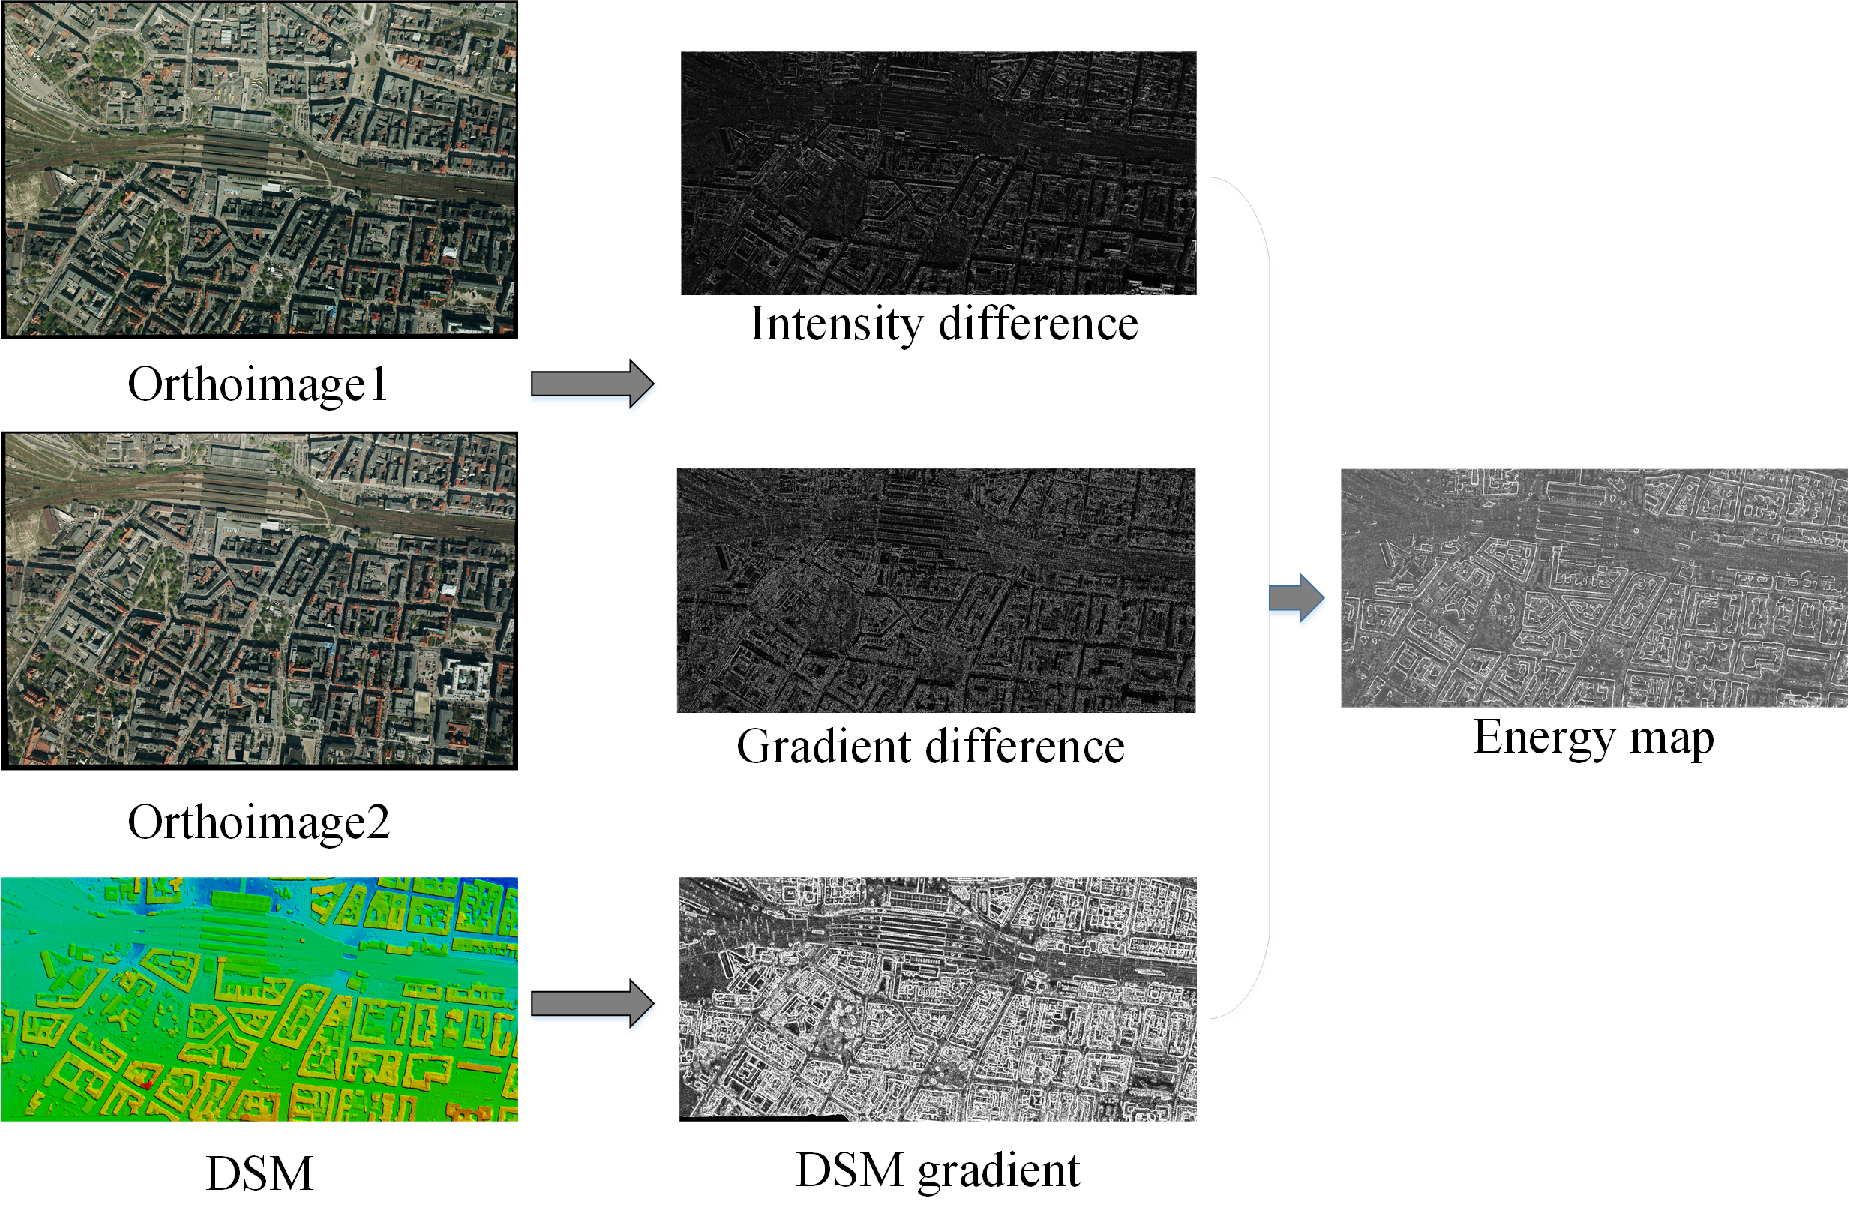
\includegraphics[width=0.5\textwidth]{energy}
	\caption{Energy map generation.}
	\label{fig:energymap}
\end{figure}
A fine seamline tends to pass through overlap area of less misalignment between adjacent orthoimages. We calculate energy for every pixel in the overlap to represent its difference on two images. Due to the ``same object with different spectrum'' and ``foreign objects with same spectra'' phenomena, auxiliary elevation information is adopted in addition to image intensity. Since DEM doesn't contain elevation information of objects above the ground level, we use DSM instead. In order to describe the difference of overlapped regions of orthoimages as objectively as possible, we extensively consider factors such as intensity difference, gradient difference, elevation gradient, etc. Energy of each pixel in the overlapping regions can be described by Eq. (\ref{eq1}):
\begin{equation}\label{eq1}
E=\alpha D_{c}+\beta D_{g}+\gamma H_{g}
\end{equation}
where $D_{c}$ represents normalized intensity difference, $D_{g}$ represents normalized gradient difference, $H_{g}$ represents normalized elevation gradient, and $\alpha$, $\beta$, $\gamma$ represent the weights for these three components respectively. Generally, the weights for color difference and gradient difference take the same value e.g. $\alpha = \beta = 1$ and the weight of elevation gradient is empirically assighed larger. e.g. $\gamma = 2$ in this paper, for we do not want the seamline pass through buildings. However, when auxiliary DSM is limited, $\gamma = 0$. As shown in Fig. \ref{fig:energymap}, the energy map can be generated by using two overlapped orthoimages and the DSM of corresponding overlap.

\subsubsection{Graph Building}
\begin{figure}[!t]
	\centering
	\includegraphics[width=0.5\textwidth]{link}
	\caption{Flowchart of the proposed graph-based mosaic algorithm.}
	\label{fig:link}
\end{figure}
Previously introduced, graph $G=\left(V, E \right)$ includes three types of nodes and edges. To build a graph, each pixel in the energy map of the buffer is regarded as a node of the graph, and the weight of the edge linking adjacent pixel nodes is defined as
\begin{equation}\label{eq2}
W_{i,j}=E_{i}+E_{j}
\end{equation}
where $E_i$, $E_j$ represent the energy value of linked pixels $i$, $j$. $W_{i,j}$ is the weight of directional edge from pixel $i$ to $j$, and $W_{i,j}=W_{j,i}$. Two adjacent images are taken as two terminals. As the Graph-cut algorithm solves the problem of pixel labeling, linking weights between pixel nodes and the $source$ and $sink$ terminals should be given. To deal with this, we adopt a nearest-neighbor strategy. For the overlap $I_S$ of two overlapped orthoimages $I_1$ and $I_2$, the linking weights between pixel nodes and terminals are
\begin{equation}\label{eq3}
S(x)= \left\{ {\begin{array}{*{20}{c}}
	{\infty,\;\;if~\forall N_{x}\notin I_{s},~N_{x}\in I_{1}}\\
	{0 ,\;\;else}
	\end{array}} \right.
\end{equation}
\begin{equation}\label{eq4}
T(x)= \left\{ {\begin{array}{*{20}{c}} 
	{\infty,\;\;if~\forall N_{x}\notin I_{s},~N_{x}\in I_{2}}\\
	{0 ,\;\;else}
	\end{array}} \right.
\end{equation}
where $N_x$ represents four-neighborhood of pixel node $x$. Eq. (\ref{eq3}) can be expressed as: if arbitrary adjacent pixel $N_x$ of $x$, which does not belong to $I_s$, belongs to $I_1$, the weight of the edge linking the $source$ and $x$ denotes infinity, otherwise it is 0. Also, Eq. (\ref{eq4}) can be expressed as: if arbitrary adjacent pixel $N_x$ of $x$, which does not belong to $I_s$, belongs to $I_2$, the weight of the edge linking sink and $x$ denotes infinity, otherwise it is 0. Thus, all elements in $G= (V, E)$ are determined. As shown in Fig. \ref{fig:link}, the buffer of two overlapped orthoimages can be mapped into a graph according to the introduced energy function and weights of linking edges.

\subsubsection{Optimizaton of Graph-cut}
Finding the min-cut of the aforementioned energy graph equals to finding the shortest seamline which passes through overlap area with least misalignment. After the graph been built, the optimization of Graph-cut is used to label the graph which minimizing the energy function of the cut. Generally, the energy function is
\begin{equation}\label{eq5}
E(L)=\sum_{x\in I_s} D(L_x)+\sum_{(x,y)\in N} W(L_x,L_y)
\end{equation}
where $L=\left \{ L_{x}\mid x\in I_s \right \}$ is labeled map of the overlapping image $I_s$, and $E(L)$ represents the loss function for the labeled map. $D$ represents loss funtion for labels. As shown in Fig. \ref{fig:link}, the weight of edge linking the source node and pixel nodes is assigned as infinite, if the pixel nodes is labeled as child node of the source terminal $S$, its loss is assigned as zero, else if it is labeled as child node of the sink terminal $T$, its loss is asigned as infinite. Namely, the node will be labeled as child node of the source terminal in any terms. $W$ represents loss function of that two adjacent nodes are labeled with different parent nodes. If two adjacent pixels are labeled with the same parent node ($S$ or $T$), $W(L_x,L_y)$ is assigned as zero, otherwise $W(L_x,L_y)$ is assigned as the weight of edge linking node $x$ and $y$.

So far, the energy function and graph needed to implement the Graph-cut algorithm have been established, and the standard Graph-cut optimization algorithm can be used to generate the labeled map, as shown in Fig. \ref{fig:link}. The mosaic image can be obtained by replacing the pixels in the overlapped area according to the labeled graph as shown in th last column of Fig. \ref{fig:link}, and the seamline can be obtained by edge detection on the labeled map. However, edge detection on the raster images will generate large number of vertices in the seamlines, we can use vector compression algorithm for optimizaiton, thus making the seamlines neat.

\subsubsection{Multi-orthoimage Mosaicking}
The mosaicking process of two orthoimages has been introduced above in detail, but in practical application, panoramic image is often obtained by multiple orthoimages. In our method, we update the effective range of orthoimages by calculating seamline with two orthoimages at a time. As shown in Fig. \ref{fig:multi-orthoimage-mosaic}, assuming that $P_1$, $P_2$, $P_3$, which are colored with red, blue and green respectively, are the effective areas of three overlapping orthoimages. Firstly, we find the seamline for $P_1$ and $P_2$, and use the resulting seamline to update effective areas as ${P_1}'$ and ${P_2}'$. Then we calculate the seamline for the updated ${P_1}'$ and $P_3$, and update the effective areas as ${P_1}''$ and ${P_3}'$. Finally, the seamline for $P_2$ and $P_3$ is obtained by their updated effective areas ${P_2}'$ and ${P_3}'$. Thus the final seamlines and effective areas for these three orthoimages are found. The gray areas in Fig. \ref{fig:multi-orthoimage-mosaic} represent mosaic buffer of overlapped orthoimages, and the black lines between two adjacent effective areas represent the final seamlines.
\begin{figure}[!t]
	\centering
	\includegraphics[width=0.45\textwidth]{mosaicking}
	\caption{Multi-orthoimage mosaicking.}
	\label{fig:multi-orthoimage-mosaic}
\end{figure}

\section{Experimental Results and Discussion}
In order to verify the validity of the proposed Graph-cut based mosaicking method, we implemented this algorithm in the 64 bit Microsoft Windows\copyright 10 operating system using C++ language in the Visual Studio 2013\copyright development environment. Our computer's key hardware configuration for running is Intel (R) Core (TM) I7 6700 quad core processor, and 16 GB memory. Testing dataset contains 69 orthoimages with the average size about $9000\times 6000$.

\subsection{Effectness Analysis}
\begin{figure}[!t]
	\centering
	\subfigure[]{\resizebox*{4.3cm}{!}{\includegraphics{photomosaic-3}}}
    \subfigure[]{\resizebox*{4.3cm}{!}{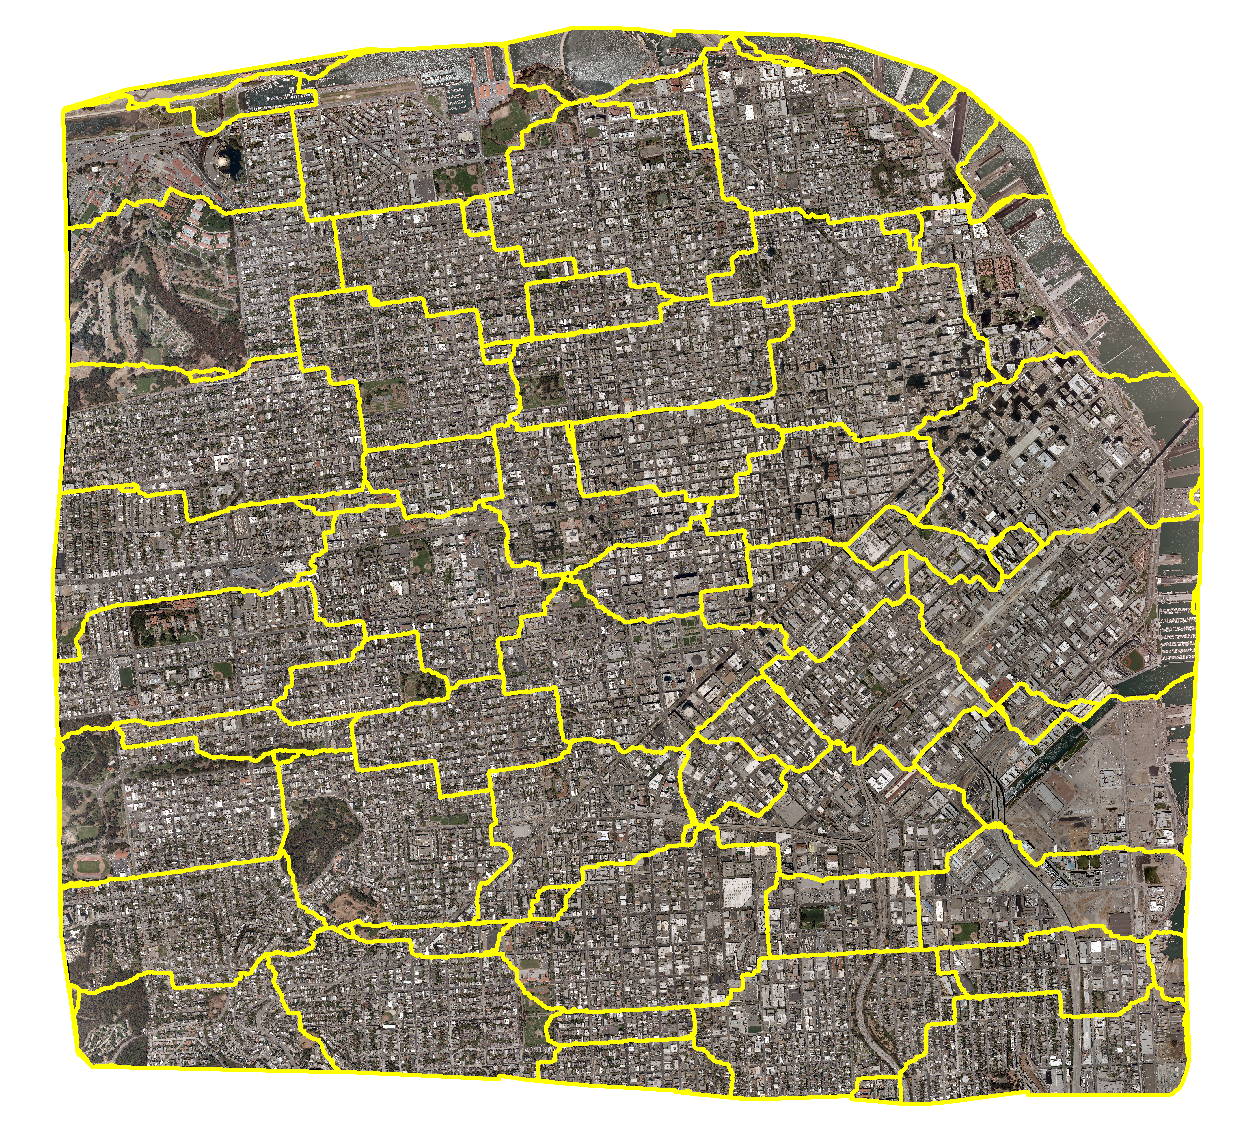
\includegraphics{photomosaic-2}}}
    \subfigure[]{\resizebox*{4.3cm}{!}{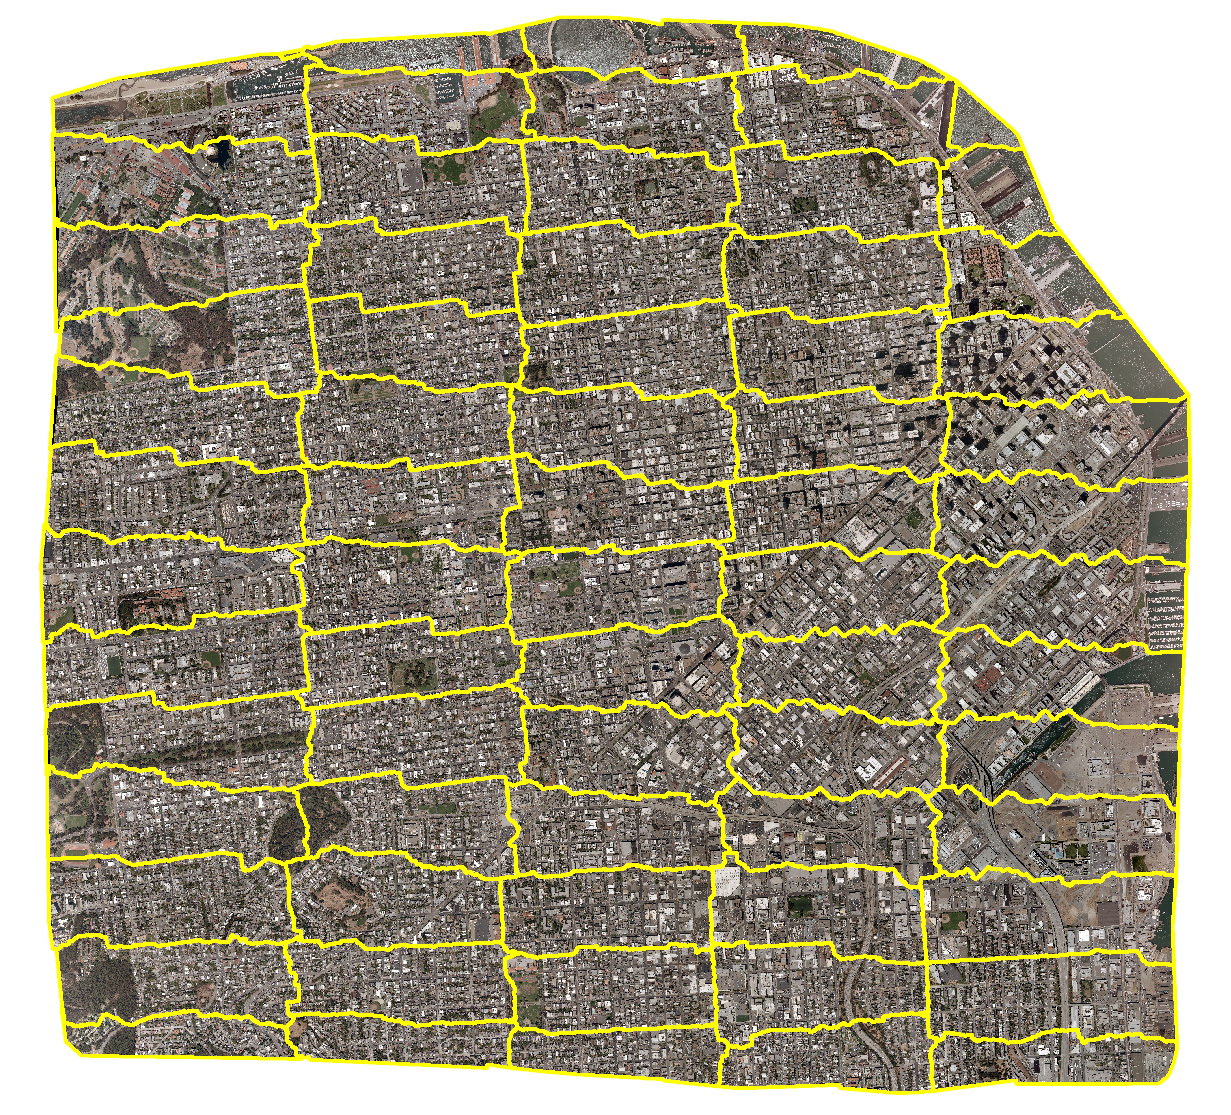
\includegraphics{photomosaic-1}}}
	\caption{Seamline network comparison: (a) seamline network obtained by the AVDO; (b) seamline network obtained by proposed method without using buffer area; (c) seamline network obtained by proposed method;  }
	\label{fig:mosaic-overall-performance}
\end{figure}

\begin{figure}[!t]
    \centering
    \subfigure[]{\resizebox*{4.3cm}{4.3cm}{\includegraphics{seamline-details-comparison-1}}}
    \subfigure[]{\resizebox*{4.3cm}{4.3cm}{\includegraphics{seamline-details-comparison-2}}}
    \subfigure[]{\resizebox*{4.3cm}{4.3cm}{\includegraphics{seamline-details-comparison-3}}}
    \subfigure[]{\resizebox*{4.3cm}{4.3cm}{\includegraphics{seamline-details-comparison-4}}}
    \caption{Seamline details comparison: (a) example 1; (b) example 2; (c) example 3; (d) example 4. The lines colored by yellow, red and green represent seamlines obtained by the AVDO method, the proposed method and the proposed method without use DSM, respectively.}
    \label{fig:seamline-details-comparison}
\end{figure}

The overall performance of the proposed method is illustrated in Fig. \ref{fig:mosaic-overall-performance}. Fig. \ref{fig:mosaic-overall-performance}(a), (b) and (c) show seamline networks obtained by the AVDO method \cite{Pan2009}, and the proposed method without and with usage of mosaic buffer, respectively. Obviously, the usage of buffer area contributes to the seamline network's regularity, which means that the effective percentage of each orthoimages in the final photomosaic is basically equivalent. There are two benefits of neat seamline network, one is easiness for further manual edit and the other is maximum usage of each orhoimages for mosaicking, for only the center of orthoimage resemble true orthoimage.

Fig. \ref{fig:seamline-details-comparison} further provides detailed comparison between results of AVDO method, and the proposed method without / with DSM's assistance, which are represented as yellow, red and green lines, respectively. As can be seen, compared to the AVDO method, the proposed method can obtain seamlines which bypass buildings efficiently and the seamline quality can be remarkably improved with auxiliary DSM. Objects like roofs which are coherent to their surrounding in color, will be easily cut through by seamlines. However, DSM can distinguish buildings from surrounding flat ground with similar texture easily. Because the energy of areas in building edges is higher than that of flat areas when DSM gradient is taken into consideration, and min-cut path will bypass such areas. The width of mosaic buffer $r$ is the key parameter of the proposed method which affect both seamline quality and time efficiency. Considering that building is the most common object above ground, the parameter $r$ is empirically assigned with the common building size, that is $60 m$ in our experiment.
\subsection{Efficiency Analysis}
If each pixel in the overlap assimilate to a node of the graph, the number of nodes in the graph will be very large for aerial orthoimages with large overlap, which will obviously lower our algorithm's efficiency. Thus, calculation of seamline can be carried out on image pyramid, which has two advantages: to speed up the calculation by reducing the number of nodes in the graph, and to make the seamline neat by reducing vertexes on the resulting seamlines.
\begin{figure}[!t]
    \centering
    \subfigure[]{\resizebox*{9cm}{!}{\includegraphics{efficiency-compare}}}
    \subfigure[]{\resizebox*{9cm}{!}{\includegraphics{passedthrough-compare}}}
    \caption{Comparison in different scale: (a) efficiency comparison; (b) quality comparison. The red and blue line respectively represent the results obtained by proposed with / without use mosaic buffer. }
    \label{fig:seamline-efficiency-comparison}
\end{figure}

The efficiency performance of the proposed method is illustrated in Fig. \ref{fig:seamline-efficiency-comparison}(a). The blue and red lines represents time consumption of the proposed method with / without use mosaic buffer in different down-sampling scale respectively. Obviously, the mosaic buffer strategy adopted by the proposed method can improve efficiency remarkably. Besides, experiments show that mosaicking in image pyramid can greatly decrease time consumption of the proposed method. Fig. \ref{fig:seamline-efficiency-comparison}(b) illustrates seamline quality of the proposed method, we count the number of obvious ground objects passed through by resulting seamlines in different image scale, which is a common criterion for seamline quality assessment. As can be seen, the seamline quality descends notably with the scale factor increases. The main reason for this phenomenon is that the building pixels and non-building pixels are blended in image pyramid, which results in seamlines passing through buildings. According to Fig. \ref{fig:seamline-efficiency-comparison}, the optimal sampling scale of the proposed method is around 1:2 to 1:4, as a trade off between efficiency and seamline quality. Table \ref{tab:quantitative-comparison} futher shows the quantitative comparison of the proposed method conducted in scale 1:3 and the AVDO method \cite{Pan2009}. As is shown that, although the AVDO method consumes less time, but its seamline quality is worse than our method, which means lots of extra manully edit is neaded for seamless photomosaic. That is to say, the proposed method is more automatic.
\newcommand{\tabincell}[2]{\begin{tabular}{@{}#1@{}}#2\end{tabular}}
\begin{table}
	\centering
	\caption{Comparison of Previous Methods and Ours.}
	\begin{tabular}[]{|c|c|c|}
		\hline
		Method &  \tabincell{c}{Number of obvious\\objects passed through} & \tabincell{c}{Processing time (s)} \\
		\hline
		AVDO \cite{Pan2014a} & \centering $>$300 &  2.2\\
		\hline	
		\tabincell{c}{Our method \\w/o mosaic buffer} &\centering 16 & 2674.0 \\
		\hline
		Our method & \centering 19 &  146.0\\
		\hline
	\end{tabular}
\label{tab:quantitative-comparison}
\end{table}

\section{Conclusion}
In this paper, a Graph-cut based aerial orthoimage mosaicking method is proposed. Image intensity and DSM are combined for energy calculation, and a strategy for graph construction is proposed. Then the Graph-cut algorithm is adopted for energy minimization and seamlines are finally generated according to graph nodes labeling. The experimental results show that the proposed method is both effective and efficient, and can effectively improve the automation of aerial orthoimage mosaicking. The proposed method can be successfully used in both traditional aerial orthoimage and UAV obtained super-high resolution orthoimage mosaicking. 

Nevertheless, the method can be further improved in serval ways: firstly, more advanced algorithms can be taken into the energy map generation procedure, such as image saliency detection and texture complexity analysis. Secondly, open-source data, such as Open Street Map, can be used as guidance for seamline searching. Thirdly, the current implementation runs in a single thread, but the multi-orthoimage mosaic procedure can be transformed to a multithreading version easily, which can dramaticly improve the time efficiency.

% Can use something like this to put references on a page
% by themselves when using endfloat and the captionsoff option.
\ifCLASSOPTIONcaptionsoff
  \newpage
\fi

{
\small
\bibliographystyle{IEEEtran}
\bibliography{Mosaic}
}
\end{document}


